\chapter{Introdução}\label{sec:introducao}

\section{Contexto}
Há décadas a comunidade científica está interessada no reconhecimento de emoções. As diversas maneiras de expressar as emoções humanas têm sido investigadas, tais como sinais fisiológicos, textos, envio de \textit{emoticons}, dispositivo padrão de entrada de dados (e.g. teclado e mouse), voz e as expressões faciais. Esta última surgiu pelas anotações de \cite{darwin1965expression} e experiências de \cite{ekman1994}. Foi percebido que todas as culturas emitem emoção pela expressão facial, de tal forma que há um grupo de emoções básicas (raiva, felicidade, tristeza, desprezo, medo e surpresa) que possuem a mesma expressão facial independente da cultura dos indivíduos. Apesar de tantos anos de pesquisa, a comunidade continua interessada neste assunto, pois reconhecer emoção tem sido desafiador. Além de ser um campo promissor para a interação humano-computador e humano-robô. Vale ressaltar que ainda é considerado um problema em aberto, inclusive com a realização de concursos com premiação, como foi o caso do ICML'2013 e anualmente como o EmotiW dos anos de 2014 a 2017.

O progresso da área de aprendizado profundo ocasionou o surgimento de diversas técnicas poderosas de reconhecimento de padrões, gerando grande destaque para as redes neurais de convolução. Esta técnica foi projetada para processamento, extração de característica e classificação de imagem. Ultimamente, as redes neurais de convolução têm sido bastantes populares e utilizadas em diversos contextos dominando amplamente os trabalhos realizados pela comunidade em classificação de imagens. Possibilitando, inclusive, o reconhecimento automático de emoção por meio da expressão facial, sendo que tal reconhecimento está próximo do que um humano reconheceria \citep{kim2016fusing}. Estes resultados expressivos têm motivado pesquisadores a continuar aprimorando estas técnicas. Sobretudo na expressão facial que tem se tornado uma abordagem eficaz para reconhecer emoções, pois não é uma abordagem intrusiva de coleta de dados quando comparada aos sensores fisiológicos. Estes sensores não são uma computação ubíqua resultando no incomodo do usuário quando seus sinais fisiológicos são monitorados. Além disso, a expressão facial possui a facilidade de ser obtida em uma captura de imagem devido a popularidade de dispositivos que possuem câmeras fotográficas \citep{cruz2017framework}.

\section{Motivação}
O reconhecimento de emoção tem aplicação em muitas áreas. Destacamos alguns campos promissores. Na educação, por exemplo, segundo \cite{jaques2013ambientes}, estudantes durante o seu processo de aprendizagem emitem constantemente diversas emoções. Portanto, sistemas educacionais como Ambientes Virtuais de Aprendizagem (AVA) e Sistemas de Tutores Inteligentes (STI) podem monitorar as emoções durante a interação com uma plataforma educacional em uma aula. Com intuito de fornecer \textit{feedback} personalizado para o estudante através da recomendação de objetos de aprendizagem apropriados para aquele estado emocional e até mesmo, realizar ações que estimulem emoções positivas a fim de motivar os estudantes quando estes estiverem em um estado negativo. Outra área de aplicação para utilizar o reconhecimento de emoção é em realidade virtual. Segundo \cite{riva2007affective}, a realidade virtual pode estimular propositalmente emoções permitindo maior imersão do usuário à aplicação. Desta forma, o reconhecimento de emoção pode medir o quão efetivo tem sido o método de estímulo de emoções ao usuário e, caso não seja satisfatório, o método pode ser alterado. Para \cite{li2015deep}, o reconhecimento de emoção pode auxiliar na construção de tecnologias assistivas para deficientes visuais que, quando possuem elevado grau de deficiência, apresentam dificuldades em reconhecer emoções na interação interpessoal. Em geral, é possível aplicar o reconhecimento de emoção na interação humano computador \citep{chen2017convolution,wen2017ensemble,liu2016facial, barsoum2016training}, e interação humano robô \citep{shin2016baseline,jung2015development}, criando a expectativa de que computadores do futuro possam reconhecer a emoção do usuário e realizar algum procedimento que ocasione maior aproximação entre homem e máquina.    

\section{Definição do Problema}\label{sec:problema}
Trata-se de um problema de classificação de imagem digital no qual há uma imagem $\omega$ formada por um conjunto de \textit{pixels} (RGB) $\alpha$ pertencente a um conjunto de classes $\sigma$ = \{neutralidade, raiva, felicidade, tristeza, desprezo, medo e surpresa\}, que são as emoções básicas definidas por \citep{ekman1994}, tal que haja uma função $\phi$ que saiba mapear $\omega$ por meio de $\alpha$ para $\sigma$.  

Embora existam trabalhos que classifiquem emoções em imagens \citep{kim2016fusing, yu2016customized,barsoum2016training}, pouca atenção tem sido dada aos problemas clássicos em imagens como: (i) ausência de iluminação no ambiente; (ii) rotação do objeto principal, neste caso a face, e (iii) escala do objeto principal (face). Abordagens que tratam estes problemas em imagens são mais apropriadas para o uso em cenários reais, no qual a exigência  para classificação é maior devido as condições adversas do ambiente e pelas diferentes variações das características da face humana. 

O problema considerado neste trabalho pode ser expresso na seguinte questão: \textit{Como aprimorar os métodos de reconhecimento de emoções por meio da expressão facial a fim de permitir a classificação independente das características do ambiente e de indivíduos para o alcance de maior generalização?} 

\section{Objetivos}

\subsection{Objetivo Geral}
Propor um método para reconhecer emoção humana por expressão facial para classificar emoções básicas em múltiplas faces de uma imagem e comparar a eficácia em cenários de uso real.
%Desenvolver um reconhecedor de emoção humana por expressão facial utilizando redes neurais de convolução para classificar as emoções básicas em múltiplas faces de uma imagem, e comparar a sua eficácia em cenários de uso real.

\subsection{Objetivos Específicos}
\begin{itemize}
 %\item Gerar um módulo de pré-processamento para eliminação de ruídos;
 %\item Propor um detector de face para recortar as diversas faces em uma imagem;
 %\item Implementar uma rede neural de convolução para em uma imagem para realizar extração de características, redução de dimensionalidade e classificação;
 \item Propor técnicas de eliminação de ruídos e detecção com recorte das diversas faces de uma imagem;
 \item Classificar cada face detectada separadamente estimando a probabilidade para cada emoção básica;
 \item Avaliar experimentalmente a solução proposta visando a comparação da eficácia.
\end{itemize}

\section{Hipótese}
As emoções básicas emitidas por expressão facial podem ser reconhecidas por uma rede neural de convolução, desde que esteja treinada e validada por instâncias representativas do problema (veja Seção \ref{sec:problema}). Além disso, este trabalho apoia-se na combinação entre a rede neural de convolução com técnicas de pré-processamento, e também, o aumento de dados durante o treinamento. Essas técnicas aplicam nas imagens: normalizações da iluminação, eliminação de ruídos, geração de novas instâncias representativas e o alinhamento da face. Com intuito de gerar modelos que maximizam a acurácia e a generalização do aprendizado relacionada ao reconhecimento de emoção em diferentes ambientes e variações da face humana.  

%Se utilizar redes neurais de convolução juntamente com técnicas de pré-processamento, aplicando transformações na imagem, como escala de cinza, filtros e redimensionamento da imagem e, realizar o mapeamento das formas presentes na imagem, como pontos relevantes da face que se alteram quando há emissão de uma determinada emoção, então, torna-se possível a classificação de emoções do usuário por meio das expressões faciais, realizando processamento digital de imagens a partir do treinamento da rede com a imagem pré-processada, focalizando na extração de características relevantes para a separação das classes. 

\section{Abordagem Proposta}\label{sec:abordagemproposta}

\subsection{Visão Geral da Solução Proposta}
Uma visão geral da solução proposta é apresentada na Figura \ref{fig:arquitetura}. Há algum dispositivo de monitoramento que contém câmera fotográfica (e.g. smartphone, notebook, televisão e outros) que periodicamente captura imagens. Toda fotografia capturada pelo dispositivo é salva em um repositório de entrada de dados. Este repositório é consultado para recuperar uma imagem e enviá-la para a classificação. No processo de classificação, é verificada a existência de uma face na imagem e, caso não exista, é encerrada a execução. Pois se trata de uma imagem que não contém uma face, portanto, não existe uma expressão facial para classificar. Caso exista uma face, uma função para recortá-la é chamada. Este procedimento é valoroso por dois aspectos: o primeiro por excluir o \textit{background} da imagem, sendo assim o classificador não necessita aprender a diferenciar o que é face e \textit{background}, e o segundo é pela possibilidade de haver múltiplas faces na imagem realizando a classificação de cada face individualmente, reduzindo a complexidade do problema, pois é mais fácil classificar uma face por vez do que várias ao mesmo tempo. Posteriormente, a face recortada é enviada a um conjunto de filtros de pré-processamento que por sua vez operam sobre a imagem para eliminação de ruídos, normalizações do contraste e alinhamento. Finalmente, a imagem pré-processada é enviada a uma rede neural de convolução para a extração de características e classificação. Esta técnica pode ter uma característica em particular que é interessante: em vez de retornar à classe a que a expressão facial (ou uma instância) pertence, pode retornar às estimativas de probabilidade para cada classe da expressão facial (e.g. neutralidade: 0.95, felicidade: 0.025, medo: 0.025,...) possuindo assim uma propriedade em que a soma das probabilidades de todas as classes é igual a 1. Sendo assim, a classificação da instância em análise seria a classe com maior probabilidade estimada (neutralidade com 0.95 de certeza). Em nossa abordagem, após a geração das estimativas de probabilidades, as mesmas são salvas em um repositório de saída de dados disponibilizando o resultado para aplicação solicitante. O processo anteriormente descrito deve ser repetido enquanto houver faces para classificar, isto é, quando uma imagem há múltiplas faces, e cada face é classificada uma por vez.

\subsection{Computação embarcada e em nuvem}
Esta proposta visa fornecer soluções para reconhecimento de emoção que contempla dois tipos de computação: em nuvem e embarcada. Tais computações estão em alta na academia, indústria e mercado. A primeira pelo crescimento da internet havendo bilhões de dispositivos conectados, e também, pela a evolução da infraestrutura com aumento considerável de recursos computacionais e velocidade de conexão. Já a computação embarcada é principalmente pela explosão de dispositivos presentes em nosso cotiano. Além disso, os dispositivos embarcados de hoje tem uma autonomia energética periódica, hardware semelhante a desktops, sistemas operacionais e sensores embutidos, formando um recurso independente e poderoso. Há no mercado vários smartphones e smartwatches com processadores octa-core e dual-core, respectivamente, com a memória RAM chegando a 8GB, e até mesmo com placas de vídeos embutidas para aceleração da computação.        

A ideia é que a computação em nuvem hospedaria o melhor modelo gerado a partir das arquiteturas AlexNet, VGGNet, GoogLeNet e Residuais, considerando as métricas de avaliação de desempenho como acurácia, precisão, revocação e f1-score. Apesar de que o melhor modelo possa exigir elevada utilização de recursos computacionais por ser uma rede neural profunda, entende-se que um serviço em nuvem possuiria um hardware robusto capaz de suportar a demanda. Visto que estamos diante do crescimento da computação cognitiva, isto é, a capacidade de computadores tomar decisões como humanos. Este trabalho quer apoiar estas aplicações oferecendo um reconhecedor de emoções para a integração em um serviço em nuvem, onde a aplicação solicitante independente da linguagem de programação esteja implementada ou em qual plataforma está rodando, possam comunicar-se via padrão REST com intuito de enviar imagens e receber as emoções detectadas.    

Em aplicações com características de computação embarcada, este trabalho propõe uma rede neural de convolução baseada na arquitetura MobileNet para funcionar nativamente em um dispositivo embarcado. Essa arquitetura tem características de ser mais enxuta sendo projetada para consumir menos recursos computacionais, e além disso, com o enxugamento possui o compromisso de perder o mínimo de precisão comparada as arquiteturas robustas. Portanto, ideal para dispositivos embarcados que dispõe de menos recursos computacionais. Inclusive podendo funcionar nativamente no sistema operacional Android que é amplamente usado por \textit{smartphones}, \textit{smartwatches} e \textit{tablets}. Além disso, a arquitetura MobileNet pode ser também embutida em placas de desenvolvimento como Raspberry, Nvidia Jetson, Drones e outras.  

Vale destacar que as maiores taxas de ocupação de recursos computacional de uma rede neural de convolução estão na fase de treinamento, isto é, durante a geração do modelo. Logo, a fase de classificação exige menores taxas de ocupação de hardware, pois o principal procedimento que demanda recursos computacionais consiste em carregar o modelo na memória. Para classificar uma imagem, considerando que o modelo está carregado na memória, a rede neural opera sobre a imagem aplicando os pesos recuperados do modelo. Os pesos configuram-se como o aprendizado retido. Em contrapartida, a fase de treinamento exige muito mais processamento, pois é executado o algoritmo de otimização gradiente descendente para minimizar a função de perda e adquirir aprendizado, realizando uma alta quantidade de cálculos vetoriais.   


\begin{figure}
\centering
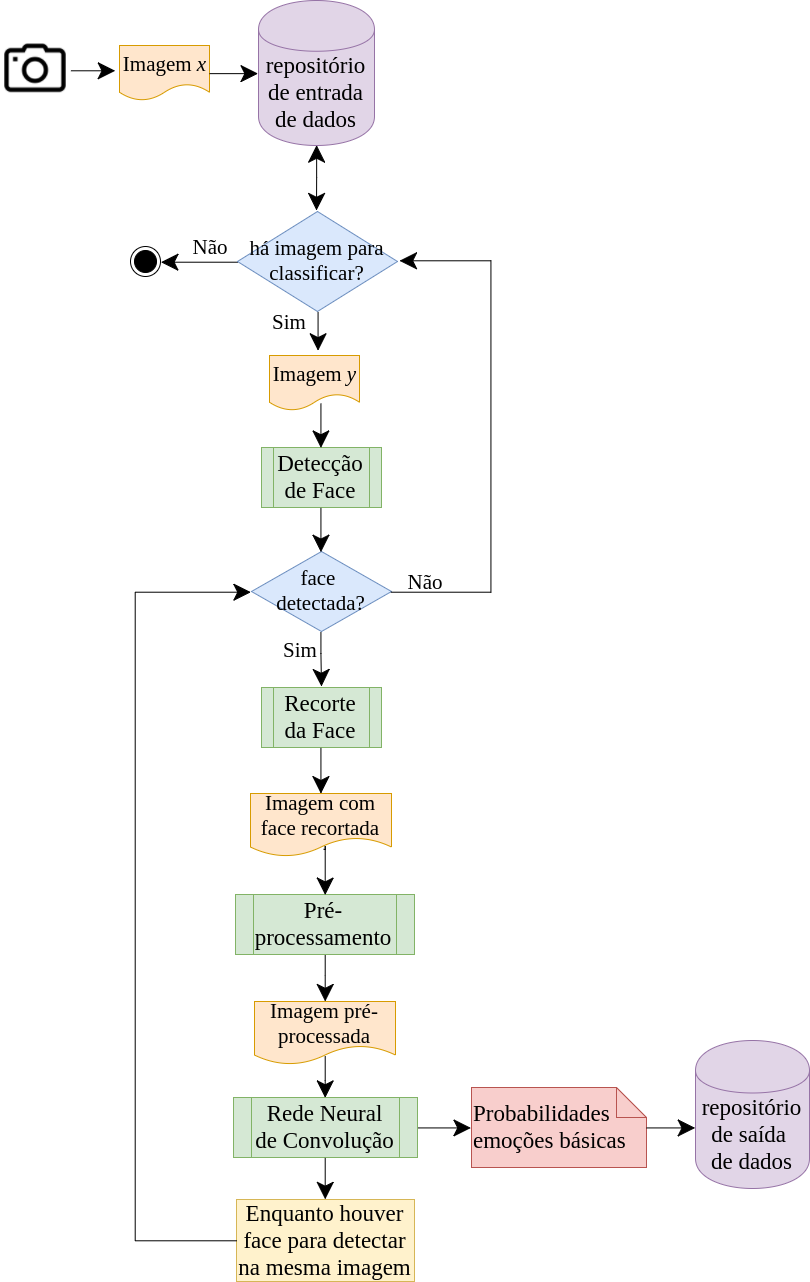
\includegraphics[scale=0.45]{figuras/arquitetura.png}
\caption{Solução Proposta}
\label{fig:arquitetura}
\end{figure}

\section{Organização do Trabalho}
Este trabalho está dividido nos capítulos a seguir. O Capítulo \ref{sec:conceitos} aborda os conceitos e definições necessários para o entendimento deste trabalho. O Capítulo \ref{sec:relacionados} analisa os trabalhos relacionados. O Capítulo \ref{sec:abordagemproposta} apresenta a abordagem proposta. O Capítulo \ref{sec:resultados} discute os resultados parciais obtidos, enquanto o Capítulo \ref{sec:conclusao} enfatiza as considerações finais, limitações do trabalhos e os trabalhos futuros.